\hypertarget{setup-local-env}{%
\chapter{アプリケーション開発の準備}\label{setup-local-env}}
\thispagestyle{frontheadings}

これまでに学んだJavaScriptの基本構文は、実行環境を問わずに使えるものです。
しかしこの後に続くユースケースの章では、具体的な実行環境としてウェブブラウザと\href{https://nodejs.org/ja/}{Node.js}\footnote{\url{https://nodejs.org/ja/}}の2つを扱います。
また、ブラウザで実行するアプリケーションであっても、その開発にはツールとしてのNode.jsが欠かせません。
このセクションではユースケースの学習へ進むために必要なアプリケーション開発環境の準備を行います。

\hypertarget{install-nodejs}{%
\section{Node.jsのインストール}\label{install-nodejs}}

\href{https://nodejs.org/ja/}{Node.js}はサーバーサイドJavaScript実行環境のひとつで、次のような特徴があります。

\begin{itemize}
\item
  ウェブブラウザのChromeと同じ\href{https://developers.google.com/v8/}{V8}
  JavaScriptエンジンで動作する
\item
  オープンソースで開発されている
\item
  OSを問わずクロスプラットフォームで動作する
\end{itemize}

Node.jsはサーバーサイドで使うために開発されました。
しかし今ではコマンドラインツールや\href{http://electron.atom.io/}{Electron}などのデスクトップアプリケーションにも利用されています。
そのため、Node.jsはサーバーサイドに限らずクライアントサイドのJavaScript実行環境としても幅広く使われています。

Node.jsは多くの他のプログラミング言語と同じように、実行環境をマシンにインストールすることで使用できます。
公式の\href{https://nodejs.org/ja/download/}{ダウンロードページ}\footnote{\url{https://nodejs.org/ja/download/}}から、開発用のマシンに合わせたインストーラをダウンロードして、インストールしましょう。

Node.jsには\textbf{LTS(Long-Term
Support)}版と最新版の2つのリリース版があります。 \textbf{LTS(Long-Term
Support)}版は2年間のメンテナンスとサポートが宣言されたバージョンです。
具体的には、後方互換性を壊さない範囲でのアップデートと、継続的なセキュリティパッチの提供が行われます。
一方で、最新版はNode.jsの最新の機能を使用できますが、常に最新のバージョンしかメンテナンスされません。
ほとんどのユーザーは、LTS版を用いることが推奨されます。Node.jsでの開発が初めてであれば、迷わずにLTS版のインストーラをダウンロードしましょう。
この章では執筆時点の最新LTS版であるバージョン12.13.0で動作するように開発します。

インストールが完了すると、コマンドラインで\texttt{node}コマンドが使用可能になっているはずです。
次のコマンドを実行して、インストールされたNode.jsのバージョンを確認しましょう
(\texttt{\$}はコマンドラインの入力欄を表す記号であるため、実際に入力する必要はありません)。

\begin{lstlisting}
$ node -v
v12.13.0
\end{lstlisting}

また、Node.jsには\href{https://www.npmjs.com/}{npm}\footnote{\url{https://www.npmjs.com/}}というパッケージマネージャーが同梱されています。
Node.jsをインストールすると、\texttt{node}コマンドだけでなくnpmを扱うための\texttt{npm}コマンドも使えるようになっています。
次のコマンドを実行して、インストールされたnpmのバージョンを確認しましょう。

\begin{lstlisting}
$ npm -v
6.12.0
\end{lstlisting}

npmや\texttt{npm}コマンドについての詳細は\href{https://docs.npmjs.com/}{公式ドキュメント}\footnote{\url{https://docs.npmjs.com/}}や\href{https://github.com/npm/cli}{npmのGitHubリポジトリ}\footnote{\url{https://github.com/npm/cli}}を参照してください。
Node.jsのライブラリのほとんどはnpmを使ってインストールできます。
実際に、ユースケースの章ではnpmを使ってライブラリをインストールして利用します。

\hypertarget{npx-execution}{%
\section{npxコマンドによるnpmパッケージの実行}\label{npx-execution}}

Node.jsを使ったコマンドラインツールは数多く公開されており、npmでインストールすることによりコマンドとして実行できるようになります。
ところで、Node.jsのインストールにより、\href{https://blog.npmjs.org/post/162869356040/introducing-npx-an-npm-package-runner}{npx}というコマンドも使えるようになっています。
\texttt{npx}コマンドを使うと、npmで公開されている実行可能なパッケージのインストールと実行をまとめてできます。
この後のユースケースでも\texttt{npx}コマンドでツールを利用するため、ここでツールの実行を試してみましょう。

ここでは例として\href{https://github.com/js-primer/hello-world}{\texttt @js-primer/hello-world}というサンプル用のパッケージを実行します。
\texttt{npx}コマンドでコマンドラインツールを実行するには、次のように
\texttt{npx}コマンドにパッケージ名を渡して実行します。

\begin{lstlisting}
$ npx @js-primer/hello-world
npx: 1個のパッケージを7.921秒でインストールしました。
Hello World!
\end{lstlisting}

このように、\texttt{npx}コマンドを使うことによりnpmで公開されているコマンドラインツールを簡単に実行できます。

\begin{tcolorbox}[title=コマンドラインツールのインストールと実行]\label{command-line-tools-installation}

npmで公開されているコマンドラインツールを実行する方法は\texttt{npx}コマンドだけではありません。
\texttt{npm install}コマンドを使ってパッケージをインストールし、インストールされたパッケージのコマンドを実行する方法があります。
通常の\texttt{npm install}コマンドは実行したカレントディレクトリにパッケージをインストールしますが、\texttt{-\/-global}フラグを加えるとパッケージをグローバルインストールします。
グローバルインストールされたパッケージのコマンドは、\texttt{node}コマンドや\texttt{npm}コマンドと同じように、任意の場所から実行できます。

次の例では\texttt{@js-primer/hello-world}パッケージをグローバルインストールしています。
その後、パッケージに含まれている\texttt{js-primer-hello-world}コマンドを絶対パスの指定なしで呼び出しています。

\begin{lstlisting}
$ npm install --global @js-primer/hello-world
$ js-primer-hello-world
Hello World!
\end{lstlisting}
\end{tcolorbox}

\hypertarget{local-server}{%
\section{ローカルサーバーのセットアップ}\label{local-server}}

「\hyperlink{read-eval-print}{値の評価と表示}」の章では、\texttt{index.html}と\texttt{index.js}というファイルを作成してブラウザで表示していました。
このときローカルに作成したHTMLファイルをそのままブラウザで読み込むと、ブラウザのアドレスバーは\texttt{file:///}からはじまるURLになります。
\texttt{file}スキーマでは\href{https://developer.mozilla.org/ja/docs/Web/Security/Same-origin_policy}{Same Origin
Policy}\footnote{\url{https://developer.mozilla.org/ja/docs/Web/Security/Same-origin_policy}}というセキュリティ的な制限により、多くの場面でアプリケーションは正しく動作しません。

これからユースケースの章で書いていくアプリケーションは、\href{https://developer.mozilla.org/ja/docs/Web/Security/Same-origin_policy}{Same Origin
Policy}の制限を避けるために、\texttt{http}スキーマのURLでアクセスすることを前提としています。
開発用のローカルサーバーを使うことで、ローカルに作成したHTMLファイルも\texttt{http}スキーマのURLで表示できます。

ここでは、これからのユースケースで利用する開発用のローカルサーバーをセットアップする方法を見ていきます。

\hypertarget{preparing-html}{%
\subsection{HTMLファイルの用意}\label{preparing-html}}

まずは最低限の要素だけを配置したHTMLファイルを作成しましょう。
ここでは\texttt{index.html}というファイル名で作成し、HTMLファイル内には次のように記述しています。
このHTMLファイルでは\texttt{script}要素を使って\texttt{index.js}というファイル名のJavaScriptファイルを読み込んでいます。

\begin{listtitle}
index.html
\end{listtitle}
\begin{lstlisting}
<html lang="ja">
  <head>
    <meta charset="utf-8" />
    <title>index.html</title>
  </head>
  <body>
    <h1>ローカルサーバで配信中</h1>
    <script src="index.js"></script>
  </body>
</html>
\end{lstlisting}
\listend

同じように\texttt{index.js}というファイル名でJavaScriptファイルを作成します。
この\texttt{index.js}には、スクリプトが正しく読み込まれたことを確認できるよう、コンソールにログを出力する処理だけを書いておきます。

\begin{listtitle}
index.js
\end{listtitle}
\begin{lstlisting}
console.log("index.js: loaded");
\end{lstlisting}
\listend

\hypertarget{open-js-primer-local-server}{%
\subsection{ローカルサーバーを起動する}\label{open-js-primer-local-server}}

先ほど作成した\texttt{index.html}と同じディレクトリで、ローカルサーバーを起動します。
次のコマンドでは、\texttt{@js-primer/local-server}というこの書籍用に作成されたローカルサーバーモジュールをダウンロードと同時に実行します。
このローカルサーバーモジュールは、\texttt{http}スキーマのURLでローカルファイルへアクセスできるように、実行したディレクトリにあるファイルを配信する機能を持ちます。

\begin{lstlisting}
# からはじまる行はコメントなので実行はしなくてよい
# cdコマンドでファイルがあるディレクトリまで移動
$ cd "index.htmlがあるディレクトリのパス"

# npx コマンドでローカルサーバーを起動
$ npx @js-primer/local-server

js-primerのローカルサーバーを起動しました。
次のURLをブラウザで開いてください。

  URL: http://localhost:3000
\end{lstlisting}

起動したローカルサーバーのURL(\texttt{http://localhost:3000})へブラウザでアクセスすると、先ほどの\texttt{index.html}の内容が表示されます。
多くのサーバーでは、\texttt{http://localhost:3000}のようにファイルパスを指定せずにアクセスすると、\texttt{index.html}を配信する機能を持っています。
\texttt{@js-primer/local-server}もこの機能を持つため、\texttt{http://localhost:3000}と\texttt{http://localhost:3000/index.html}のどちらのURLも同じ\texttt{index.html}を配信しています。

\begin{figure}[h]
\centering
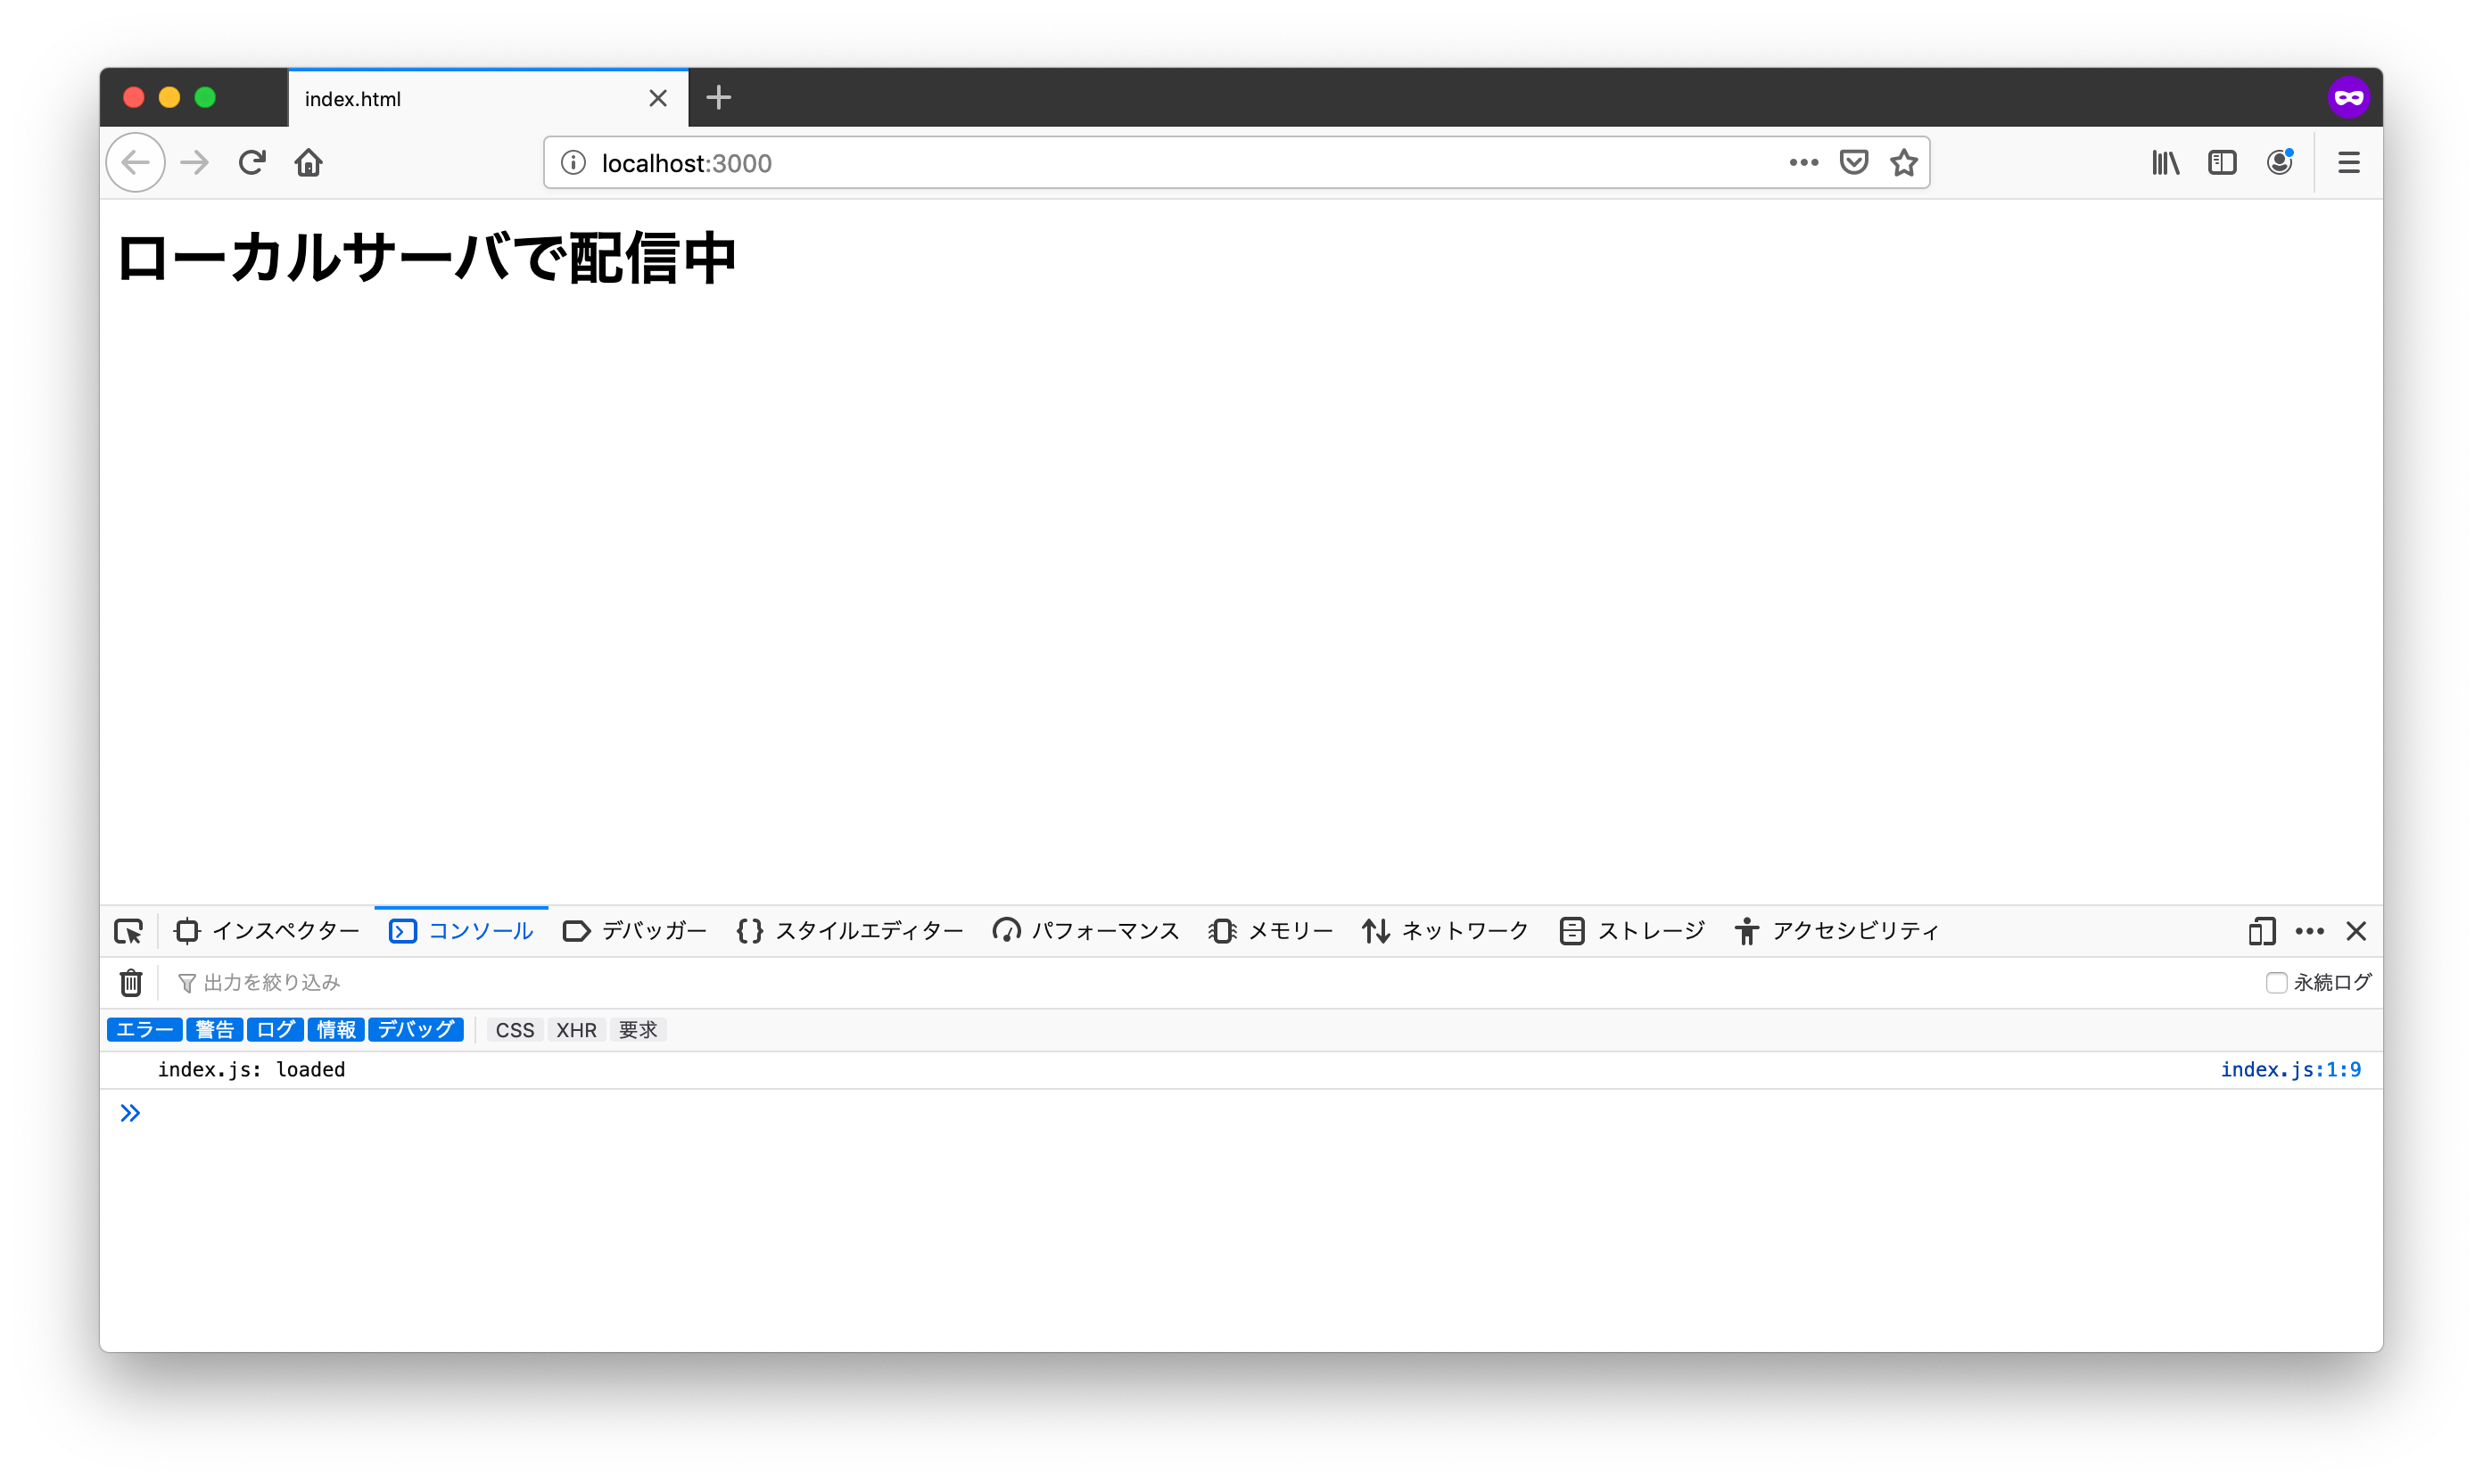
\includegraphics[width=120mm]{fig/index.png}
\caption{ログが表示されているWebコンソール}
\end{figure}

\texttt{index.html}にアクセスできたら、正しく\texttt{index.js}が読み込まれているかを確認してみましょう。
Console
APIで出力したログを確認するには、ウェブブラウザの開発者ツールを開く必要があります。
ほとんどのブラウザで開発者ツールが同梱されていますが、この書籍ではFirefoxを使って確認します。

Firefoxの開発者ツールは次のいずれかの方法で開きます。

\begin{itemize}
\item
  Firefoxメニュー(メニューバーがある場合やmacOS
  では、ツールメニュー)のウェブ開発サブメニューで``ウェブコンソール''
  を選択する
\item
  キーボードショートカット\keytop{Ctrl}+\keytop{Shift}+\keytop{K}(macOSでは
  \keytop{Command}+\keytop{Option}+\keytop{K})を押下する
\end{itemize}

詳細は``\href{https://developer.mozilla.org/ja/docs/Tools/Web_Console/Opening_the_Web_Console}{ウェブコンソールを開く}''\footnote{\url{https://developer.mozilla.org/ja/docs/Tools/Web_Console/Opening_the_Web_Console}}を参照してください。

\hypertarget{close-js-primer-local-server}{%
\subsection{ローカルサーバーを終了する}\label{close-js-primer-local-server}}

最後に、起動したローカルサーバーを終了します。
ローカルサーバーを起動したコマンドラインで、\keytop{Ctrl}+\keytop{C}を押下することで終了できます。

複数のローカルサーバーを同時に起動することも可能ですが、複数のサーバーで同じポート番号を利用することはできません。
ポートとは、先ほど起動したローカルサーバーのURLで\texttt{:3000}となっていた部分のことで、これは3000番ポートでローカルサーバーを起動したことを意味しています。

\texttt{@js-primer/local-server}は、デフォルトのポート(3000番ポート)がすでに使用されているなら、使われていないポートを探してローカルサーバーを起動します。また、\texttt{-\/-port}オプションで任意のポート番号でローカルサーバーを起動できます。

\begin{lstlisting}
$ npx @js-primer/local-server --port 8000
\end{lstlisting}

この書籍では、\texttt{@js-primer/local-server}をデフォルトのポート番号である3000番ポートを利用する前提で進めていきます。
使わなくなったローカルサーバーは\keytop{Ctrl}+\keytop{C}で終了しておくことで、アクセスするURL(ポート番号)が書籍と同じ状態で進められます。

\hypertarget{conslusion}{%
\section{まとめ}\label{conslusion}}

この章では、これからのユースケースの章で必要な環境を準備しました。

\begin{itemize}
\item
  Node.jsのLTS版をインストールした
\item
  npmとnpxでモジュールのインストールと実行をした
\item
  \texttt{@js-primer/local-server}モジュールを使ってローカルサーバーを起動して終了した
\end{itemize}

npmでは、すでに多種多様なローカルサーバーモジュールが公開されています。
この書籍では、利用するローカルサーバーの機能で違いが出ないように\texttt{@js-primer/local-server}というこの書籍用のローカルサーバーモジュールを利用します。
